\documentclass[12pt,a4paper,oneside]{article}
\usepackage[utf8]{inputenc}
\usepackage[english]{babel}
\usepackage{amsmath}
\usepackage{amsfonts}
\usepackage{amssymb}
\usepackage{graphicx}
\usepackage{multirow}
\usepackage{longtable}
\usepackage[left=3cm,right=2cm,top=3cm,bottom=2cm]{geometry}
\begin{document}

\begin{center}
\textbf{\large{Context Description and Next Activities}}
\end{center}
\bigskip

\begin{figure}[b!]
\center
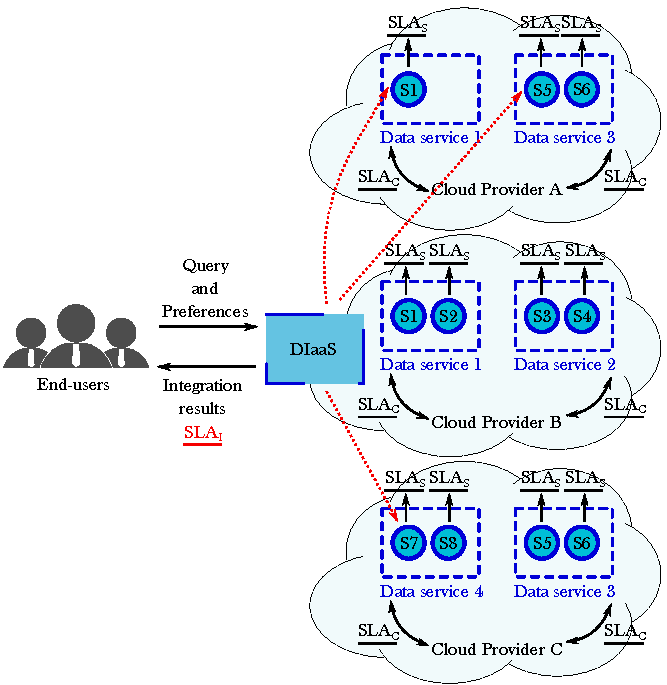
\includegraphics[scale=1]{figures/scenario.pdf}\caption{Data integration context overview}\label{fig:context}
\end{figure}

The figure~\ref{fig:context} illustrates our data integration scenario. Cloud providers (for instance, Cloud Provider A, Cloud Provider B and Cloud Provider C) offer cloud resources to data providers (for instance, Data provider 1, Data provider 2, Data provider 3 and Data provider 4) willing to deploy their services. The cloud provider and the data service establish a contract specifying what guarantees in terms of infrastructure resources (for instance, storage limit, memory limit, processing capacity) the data service can expect from the cloud. This contract is called \textsl{Cloud SLA} ($SLA_{C}$).

Data services can deploy services in the clouds they have subscriptions respecting what is agreed in the $SLA_{C}$. Each service deployed by the data service in the cloud export a different SLA (called \textsl{Service SLA} - $SLA_{S}$) which specifies what service customers can expect in terms of data quality guarantees (for instance, provenance, freshness, data type, degree of rawness) from its service. The data provider defines the $SLA_{S}$ for the services deployed on a cloud according to what it is defined in the $SLA_{C}$. For instance, considering that a \textsl{data provider} have agreed with a \textsl{cloud provider} to have limit of 10 gigabytes of free data transferred per day, the \textsl{data provider} could define on his $SLA_{S}$ that he can perform 300 requests per day, and each request costs 0.1\$. In other words, the $SLA_{S}$ guarantees are derived from the $SLA_{C}$. Moreover, a \textsl{data provider} can deploy the same service in different clouds in which he has established contracts (for instance, the \textsl{Data provider} 1 deployed the service S1 in the clouds A and B) and for each different \textsl{Cloud provider} a different $SLA_{S}$ is defined for the same service.

The end-user willing to integrate data interacts with our \textsl{Data Integration-as-a-Service} (\textsl{DIaaS}). The \textsl{DIaaS} is responsible to select and match the services that can produce the result expected by the user according to his preferences, where he is consuming the data, and the different SLAs associated to the services and to the cloud providers. Once the composition is created and executed, the integration results are delivered to the user and an \textsl{integration SLA} ($SLA_{I}$) is established. This SLA is responsible to include information collected during the integration process which can be reused in a further integration request.

\paragraph{Activities for the next meeting:}
\begin{enumerate}
\item Enumerate the possible cases of queries and their variations to be able to identify what could be of interest to be in the \textsl{integration SLA} and what information should I collect in the integration process.
\item Propose the schemas of $SLA_{C}$ and $SLA_{S}$ according to the schema that I have removing what is not necessary for it (clauses extraction from SLA and how those clauses will feed the rewriting algorithm: study all the cases: clauses are compatibles, clauses are partially compatible...etc).
\end{enumerate}


\begin{flushleft}
\textbf{List of query variations}
\end{flushleft}

% Please add the following required packages to your document preamble:
% \usepackage{multirow}
%\begin{table}[]
\begin{center}
\begin{longtable}{|l|p{8cm}|}
%%%
  %%% firsthead -- essa seção aparece apenas no primeiro cabeçalho.
  %%%
  \hline
  \textbf{Query} & \textbf{Requirements} \\
  \hline\hline
  \endfirsthead
  %%%
  %%% head -- essa seção aparece nos demais cabeçalhos.
  %%%
  %\caption[]{Exemplo de uma tabela muito longa (continuação)} \\
  \hline
  \textbf{Query} & \textbf{Requirements} \\
  \hline\hline
  \endhead
  %%%
  %%% lastfoot -- essa seção aparece apenas no último rodapé.
  %%%
  %\hline %\hline
  \endlastfoot
  %%%
  %%% foot -- essa seção aparece nos demais rodapés.
  %%%
%  \hline
%  \multicolumn{2}{r}{\footnotesize{}continua na próxima página} \\
%  \endfoot

%                \textbf{Query}  &  \textbf{Requirements} \\ \hline
\multirow{7}{6cm}{The incoming query is the same as a previous query}  & Same requirements \\ \cline{2-2} 
                  & Requirements more restrict \\ \cline{2-2} 
                  & Requirements less restrict \\ \cline{2-2} 
                  & Part of the requirements more restrict and part of the requirements less restrict \\ \cline{2-2} 
                  & Part of the requirements more restrict and part of the requirements different \\ \cline{2-2} 
                  & Part of the requirements less restrict and part of the requirements different \\ \cline{2-2} 
                  & Requirements completely different \\ \hline
\multirow{7}{6cm}{The incoming query is a subset of a previous query}  &Same requirements \\ \cline{2-2} 
                  & Requirements more restrict \\ \cline{2-2} 
                  & Requirements less restrict \\ \cline{2-2} 
                  & Part of the requirements more restrict and part of the requirements less restrict \\ \cline{2-2} 
                  & Part of the requirements more restrict and part of the requirements different \\ \cline{2-2} 
                  & Part of the requirements less restrict and part of the requirements different \\ \cline{2-2} 
                  & Requirements completely different \\ \hline
\multirow{7}{6cm}{The previous query is a subset of the incoming query}  & Same requirements \\ \cline{2-2} 
                  & Requirements more restrict \\ \cline{2-2} 
                  & Requirements less restrict \\ \cline{2-2} 
                  & Part of the requirements more restrict and part of the requirements less restrict \\ \cline{2-2} 
                  & Part of the requirements more restrict and part of the requirements different \\ \cline{2-2} 
                  & Part of the requirements less restrict and part of the requirements different \\ \cline{2-2} 
                  & Requirements completely different \\ \hline
\multirow{7}{6cm}{Different queries but the incoming query has some abstract services in common with the previous query}  & Same requirements \\ \cline{2-2} 
                  & Requirements more restrict \\ \cline{2-2} 
                  & Requirements less restrict \\ \cline{2-2} 
                  & Part of the requirements more restrict and part of the requirements less restrict \\ \cline{2-2} 
                  & Part of the requirements more restrict and part of the requirements different \\ \cline{2-2} 
                  & Part of the requirements less restrict and part of the requirements different \\ \cline{2-2} 
                  & Requirements completely different \\ \hline
\multirow{7}{6cm}{Different queries} & Same requirements \\ \cline{2-2} 
                  & Requirements more restrict \\ \cline{2-2} 
                  & Requirements less restrict \\ \cline{2-2} 
                  & Part of the requirements more restrict and part of the requirements less restrict \\ \cline{2-2} 
                  & Part of the requirements more restrict and part of the requirements different \\ \cline{2-2} 
                  & Part of the requirements less restrict and part of the requirements different \\ \cline{2-2} 
                  & Requirements completely different \\ \hline
\caption{List of possible query variations\label{tab:big}} \\
\end{longtable}%\caption{My caption}\label{my-label}
\end{center}

\begin{flushleft}
\textbf{Cloud SLA} (Figure~\ref{fig:cloudsla})
\end{flushleft}

\begin{figure}[h!]
\center
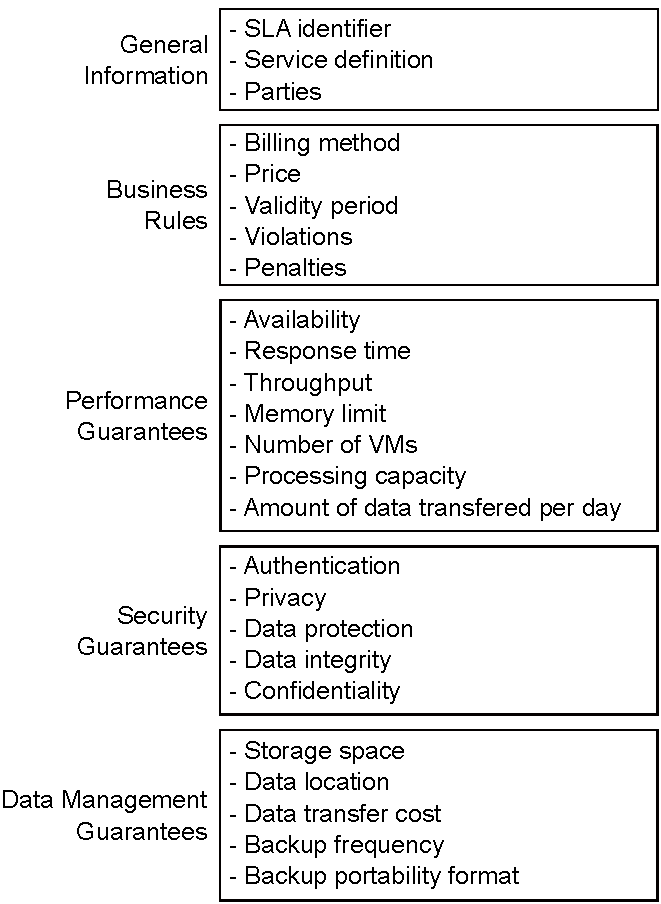
\includegraphics[scale=1]{figures/Cloud-SLA-Schema.pdf}\caption{Cloud SLA schema}\label{fig:cloudsla}
\end{figure}

\begin{flushleft}
\textbf{Service SLA} (Figure~\ref{fig:servicesla})
\end{flushleft}

\begin{figure}[h!]
\center
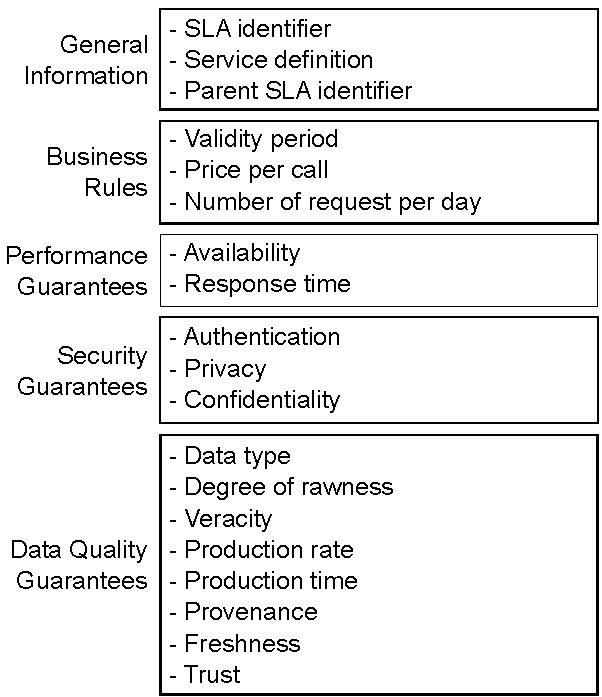
\includegraphics[scale=1]{figures/Service-SLA-Schema.pdf}\caption{Service SLA schema}\label{fig:servicesla}
\end{figure}


\begin{flushleft}
\textbf{Integration SLA}
\end{flushleft}

By considering the list of query variations, the following clauses are interesting to be part of the \textsl{integration SLA} in order to optimize a further integration request. 

\begin{enumerate}
\item \textit{The complete query definition}. The query is necessary to identify similarities with a further integration request.
\item \textit{The list of user preferences}. The \textsl{user preferences} are necessary to identify similarities with a further integration request.
\item \textit{Integration total cost}. The integration final cost could be a \textsl{user preferences} being used a filtering measure.
\item \textit{Integration time}. The necessary time to perform the integration process. This could be a filtering measure considering the \textsl{user preferences}.
\item \textit{Used data services}. The \textsl{data services} that were used in a previous integration process.
\item \textit{User data consumption environment}. The environment that the user is using to consume the data.
\item \textit{Amount of data transferred}. The amount of data that were transferred and delivered to the user.
\item \textit{Consumption time}. The time necessary to deliver the results to the user considering his consumption environment. 
\end{enumerate}

The following information seems to be interest for the integration process. However, it is not an information to be included in the \textsl{integration SLA} once it is something general for every integration request. I believe it should be included in a file apart.

\begin{flushleft}
\textbf{\textsl{Abstract services} description} (I do not know if it is the best name for it): it is a file that associates an \textsl{abstract service} to \textsl{data services} that can answer to it including performance information of the \textsl{data service}.
\end{flushleft}

This file should include the information regarding the \textsl{data services} that can cover an \textsl{abstract service}. In the case when no reusable integration exists, this file would avoid the effort of searching for \textsl{data services} that can cover an \textsl{abstract service} when a new integration request arrives. Even in the case when a reusable integration exists, it could help while identifying and substituting \textsl{data services} that are not good in performance or that are not interest considering the current \textsl{user preferences}, for instance. Moreover, during the integration process information concerning the processing time of each involved \textsl{data service} is collected and included in this file. This information could be interest while choosing a \textsl{data services} for a further integration process.

\end{document}